\documentclass[aspectratio=169, 10pt]{beamer}

% 导言区设置
\usepackage[utf8]{inputenc}
\usepackage{ctex}
\usepackage{amsmath, amssymb}
\usepackage{pgfplots}
\pgfplotsset{compat=1.18}
\usepackage{xcolor}
\usepackage{tcolorbox}

% 自定义颜色
\definecolor{myblue}{RGB}{0, 112, 192}
\definecolor{myorange}{RGB}{237, 125, 49}
\definecolor{mygreen}{RGB}{0, 176, 80}

% Beamer 主题设置
\usetheme{Madrid}
\usecolortheme{beaver}
\usefonttheme{serif}
% 自定义思考框
\newtcolorbox{thinkbox}[1][]{
	colback=myorange!10,
	colframe=myorange,
	fonttitle=\bfseries,
	title={? 思考},
	arc=2mm,
	#1
}

\AtBeginSection[]
{
	\begin{frame}<beamer>
		\frametitle{本节主要内容}
		\tableofcontents[currentsection,currentsubsection]
	\end{frame}
}

\AtBeginDocument{
	\setlength{\abovedisplayskip}{3pt}
	\setlength{\belowdisplayskip}{3pt}
	\setbeamertemplate{theorems}[numbered]
}

\title{3.2.1 单调性与最大（小）值}
\author{好好学习，努力向上}
\date{}

\begin{document}
	\begin{frame}{}
		\titlepage
	\end{frame}
	
%	\begin{frame}{内容概览}
%		\tableofcontents
%	\end{frame}
	% ---------------------------------------------------------
	% 概念引入 Frame 1
	% ---------------------------------------------------------
	\begin{frame}{3.2.1 单调性与最大（小）值}
		在初中，我们利用函数图象研究过函数值随自变量的增大而增大（或减小）的性质，这一性质叫做函数的\textbf{单调性}. 下面进一步用符号语言刻画这种性质.
		
		先研究二次函数 \(f(x)=x^2\) 的单调性.
		
		\begin{columns}
			\begin{column}{0.55\textwidth}
				画出它的图象（如图），可以看到：\\
				图象在 \(y\) 轴左侧部分从左到右是下降的，也就是说，当 \(x \leqslant 0\) 时，\(y\) 随 \(x\) 的增大而减小. 用符号语言描述，就是任意取 \(x_1, x_2 \in (-\infty, 0]\)，得到 \(f(x_1)=x_1^2\)，\(f(x_2)=x_2^2\)，那么当 \(x_1 < x_2\) 时，有 \(f(x_1) > f(x_2)\). 这时我们就说函数 \(f(x)=x^2\) 在区间 \((-\infty, 0]\) 上是\textbf{单调递减}的.
			\end{column}
			\begin{column}{0.45\textwidth}
				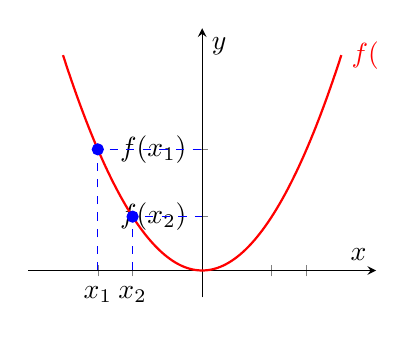
\begin{tikzpicture}
					\begin{axis}[
						axis lines=middle,
						xlabel={\(x\)}, ylabel={\(y\)},
						xmin=-2.5, xmax=2.5, ymin=-0.5, ymax=4.5,
						xtick={-1.5,-1,0,1,1.5},
						xticklabels={\(x_1\),\(x_2\),\(O\),,,},
						ytick={1,2.25},
						yticklabels={\(f(x_2)\),\(f(x_1)\)},
						width=6cm, height=5cm,
						samples=100
						]
						\addplot[thick, red, domain=-2:2] {x^2} node[right] {\(f(x)=x^2\)};
						\addplot[dashed, blue] coordinates {(-1.5, 0) (-1.5, 2.25) (0, 2.25)};
						\addplot[dashed, blue] coordinates {(-1, 0) (-1, 1) (0, 1)};
						\addplot[only marks, mark=*, blue] coordinates {(-1.5, 2.25) (-1, 1)};
					\end{axis}
				\end{tikzpicture}
			\end{column}
		\end{columns}
	\end{frame}
	
	% ---------------------------------------------------------
	% 概念引入 Frame 2
	% ---------------------------------------------------------
	\begin{frame}{单调性的符号语言刻画}
		图象在 \(y\) 轴右侧部分从左到右是上升的，也就是说，当 \(x \geqslant 0\) 时，\(y\) 随 \(x\) 的增大而增大. 用符号语言表达，就是任意取 \(x_1, x_2 \in [0, +\infty)\)，得到 \(f(x_1)=x_1^2\)，\(f(x_2)=x_2^2\)，那么当 \(x_1 < x_2\) 时，有 \(f(x_1) < f(x_2)\). 这时我们就说函数 \(f(x)=x^2\) 在区间 \([0, +\infty)\) 上是\textbf{单调递增}的.
		
		\vspace{0.5cm}
		\begin{thinkbox}
			你能说明为什么 \(f(x_1) < f(x_2)\) 吗？\\
			函数 \(f(x)=|x|\)，\(f(x)=-x^2\) 各有怎样的单调性？
		\end{thinkbox}
		
		\vspace{0.5cm}
		一般地，设函数 \(f(x)\) 的定义域为 \(D\)，区间 \(I \subseteq D\)：
		\begin{itemize}
			\item 如果 \(\forall x_1, x_2 \in I\)，当 \(x_1 < x_2\) 时，都有 \(f(x_1) < f(x_2)\)，那么就称函数 \(f(x)\) 在区间 \(I\) 上\textbf{单调递增}.
			\item 如果 \(\forall x_1, x_2 \in I\)，当 \(x_1 < x_2\) 时，都有 \(f(x_1) > f(x_2)\)，那么就称函数 \(f(x)\) 在区间 \(I\) 上\textbf{单调递减}.
		\end{itemize}
		如果函数 \(y=f(x)\) 在区间 \(I\) 上单调递增或单调递减，那么就说函数在这一区间具有（严格的）单调性，区间 \(I\) 叫做单调区间.
	\end{frame}
	
	% ---------------------------------------------------------
	% 例 1
	% ---------------------------------------------------------
	\begin{frame}{例 1：一次函数的单调性}
		\textbf{\textcolor{myblue}{例 1}} 根据定义，研究函数 \(f(x)=kx+b(k \neq 0)\) 的单调性.
		
		\vspace{0.2cm}
		\textbf{\textcolor{myorange}{分析：}}根据函数单调性的定义，需要考察当 \(x_1 < x_2\) 时，\(f(x_1) < f(x_2)\) 还是 \(f(x_1) > f(x_2)\). 根据实数大小关系的基本事实，只要考察 \(f(x_1) - f(x_2)\) 与 \(0\) 的大小关系.
		
		\vspace{0.2cm}
		\textbf{\textcolor{myblue}{解：}}函数 \(f(x)=kx+b(k \neq 0)\) 的定义域是 \(\mathbb{R}\). \(\forall x_1, x_2 \in \mathbb{R}\)，且 \(x_1 < x_2\)，则
		\begin{align*}
			f(x_1) - f(x_2) &= (kx_1 + b) - (kx_2 + b) \\
			&= k(x_1 - x_2).
		\end{align*}
		由 \(x_1 < x_2\)，得 \(x_1 - x_2 < 0\). 所以
		\begin{itemize}
			\item ①当 \(k > 0\) 时，\(k(x_1 - x_2) < 0\). 于是 \(f(x_1) - f(x_2) < 0\)，即 \(f(x_1) < f(x_2)\). 这时，\(f(x)=kx+b\) 是增函数.
			\item ②当 \(k < 0\) 时，\(k(x_1 - x_2) > 0\). 于是 \(f(x_1) - f(x_2) > 0\)，即 \(f(x_1) > f(x_2)\). 这时，\(f(x)=kx+b\) 是减函数.
		\end{itemize}
	\end{frame}
	
	% ---------------------------------------------------------
	% 例 2
	% ---------------------------------------------------------
	\begin{frame}{例 2：物理学中的玻意耳定律}
		\textbf{\textcolor{myblue}{例 2}} 物理学中的玻意耳定律 \(p=\frac{k}{V}\)（\(k\) 为正常数）告诉我们，对于一定量的气体，当其体积 \(V\) 减小时，压强 \(p\) 将增大. 试对此用函数的单调性证明.
		
		\vspace{0.2cm}
		\textbf{\textcolor{myorange}{分析：}}根据题意，只要证明函数 \(p=\frac{k}{V}\)（\(V \in (0, +\infty)\)）是减函数即可.
		
		\vspace{0.2cm}
		\textbf{\textcolor{myblue}{证明：}}\(\forall V_1, V_2 \in (0, +\infty)\)，且 \(V_1 < V_2\)，则
		\[
		p_1 - p_2 = \frac{k}{V_1} - \frac{k}{V_2} = k\frac{V_2 - V_1}{V_1V_2}.
		\]
		由 \(V_1, V_2 \in (0, +\infty)\)，得 \(V_1V_2 > 0\)；\\
		由 \(V_1 < V_2\)，得 \(V_2 - V_1 > 0\).\\
		又 \(k > 0\)，于是
		\[
		p_1 - p_2 > 0,
		\]
		即
		\[
		p_1 > p_2.
		\]
		所以，根据函数单调性的定义，函数 \(p=\frac{k}{V}\)，\(V \in (0, +\infty)\) 是减函数. 也就是说，当体积 \(V\) 减小时，压强 \(p\) 将增大.
	\end{frame}
	
	% ---------------------------------------------------------
	% 例 3
	% ---------------------------------------------------------
	\begin{frame}{例 3：利用定义证明单调性}
		\textbf{\textcolor{myblue}{例 3}} 根据定义证明函数 \(y=x+\frac{1}{x}\) 在区间 \((1, +\infty)\) 上单调递增.
		
		\vspace{0.2cm}
		\textbf{\textcolor{myblue}{证明：}}\(\forall x_1, x_2 \in (1, +\infty)\)，且 \(x_1 < x_2\)，有
		\begin{align*}
			y_1 - y_2 &= \left(x_1 + \frac{1}{x_1}\right) - \left(x_2 + \frac{1}{x_2}\right) = (x_1 - x_2) + \left(\frac{1}{x_1} - \frac{1}{x_2}\right) \\
			&= (x_1 - x_2) + \frac{x_2 - x_1}{x_1x_2} = \frac{x_1 - x_2}{x_1x_2}(x_1x_2 - 1).
		\end{align*}
		由 \(x_1, x_2 \in (1, +\infty)\)，得 \(x_1 > 1\)，\(x_2 > 1\).\\
		所以 \(x_1x_2 > 1\)，\(x_1x_2 - 1 > 0\).\\
		又由 \(x_1 < x_2\)，得 \(x_1 - x_2 < 0\).\\
		于是
		\[
		\frac{x_1 - x_2}{x_1x_2}(x_1x_2 - 1) < 0,
		\]
		即
		\[
		y_1 < y_2.
		\]
		所以，函数 \(y=x+\frac{1}{x}\) 在区间 \((1, +\infty)\) 上单调递增.
	\end{frame}
	
	% ---------------------------------------------------------
	% 练习 1
	% ---------------------------------------------------------
	\begin{frame}{练习 1：生产效率与工人数}
		\textbf{\textcolor{myblue}{1.}} 请根据下图描述某装配线的生产效率与生产线上工人数量间的关系.
		
		\begin{columns}
			\begin{column}{0.5\textwidth}
				\begin{tikzpicture}
					\begin{axis}[
						axis lines=middle,
						xlabel={工人数}, ylabel={生产效率},
						xmin=0, xmax=6, ymin=0, ymax=5,
						xtick=\empty, ytick=\empty,
						width=6cm, height=4.5cm,
						samples=100
						]
						% 使用平滑曲线模拟图像
						\addplot[thick, red, smooth, domain=0.5:5] {3*sin((x-0.5)*40)+1.5};
						\node at (axis cs:0,0) [below left] {\(O\)};
					\end{axis}
				\end{tikzpicture}
			\end{column}
			\begin{column}{0.5\textwidth}
				\textbf{解答：}\\
				由图象可知，该函数图象先上升后下降。
				\begin{itemize}
					\item 在生产线上工人数量较少时（图象左侧），随着工人数量的增加，生产效率逐渐提高（单调递增）。
					\item 当工人数量达到一定值后（图象右侧），继续增加工人数量，生产效率反而会降低（单调递减）。
				\end{itemize}
				这说明并不是工人越多越好，存在一个最佳工人数量使生产效率最高。
			\end{column}
		\end{columns}
	\end{frame}
	
	% ---------------------------------------------------------
	% 练习 2
	% ---------------------------------------------------------
	\begin{frame}{练习 2：证明一次函数单调性}
		\textbf{\textcolor{myblue}{2.}} 根据定义证明函数 \(f(x)=3x+2\) 是增函数.
		
		\vspace{0.5cm}
		\textbf{解答：}\\
		函数 \(f(x)=3x+2\) 的定义域为 \(\mathbb{R}\)。
		
		任取 \(x_1, x_2 \in \mathbb{R}\)，且 \(x_1 < x_2\)，则：
		\begin{align*}
			f(x_1) - f(x_2) &= (3x_1 + 2) - (3x_2 + 2) \\
			&= 3x_1 - 3x_2 \\
			&= 3(x_1 - x_2).
		\end{align*}
		因为 \(x_1 < x_2\)，所以 \(x_1 - x_2 < 0\)。
		又因为 \(3 > 0\)，所以 \(3(x_1 - x_2) < 0\)，即：
		\[
		f(x_1) - f(x_2) < 0.
		\]
		从而 \(f(x_1) < f(x_2)\)。
		
		根据函数单调性的定义，函数 \(f(x)=3x+2\) 在 \(\mathbb{R}\) 上是增函数。
	\end{frame}
	
	% ---------------------------------------------------------
	% 练习 3
	% ---------------------------------------------------------
	\begin{frame}{练习 3：证明反比例函数单调性}
		\textbf{\textcolor{myblue}{3.}} 证明函数 \(f(x)=-\frac{2}{x}\) 在区间 \((-\infty, 0)\) 上单调递增.
		
		\vspace{0.5cm}
		\textbf{解答：}\\
		任取 \(x_1, x_2 \in (-\infty, 0)\)，且 \(x_1 < x_2\)，则：
		\begin{align*}
			f(x_1) - f(x_2) &= \left(-\frac{2}{x_1}\right) - \left(-\frac{2}{x_2}\right) \\
			&= -\frac{2}{x_1} + \frac{2}{x_2} \\
			&= \frac{-2x_2 + 2x_1}{x_1x_2} \\
			&= \frac{2(x_1 - x_2)}{x_1x_2}.
		\end{align*}
		因为 \(x_1, x_2 \in (-\infty, 0)\)，所以 \(x_1x_2 > 0\)。
		因为 \(x_1 < x_2\)，所以 \(x_1 - x_2 < 0\)。
		因此，\(\frac{2(x_1 - x_2)}{x_1x_2} < 0\)，即 \(f(x_1) - f(x_2) < 0\)。
		所以 \(f(x_1) < f(x_2)\)。
		
		根据函数单调性的定义，函数 \(f(x)=-\frac{2}{x}\) 在区间 \((-\infty, 0)\) 上单调递增。
	\end{frame}
	
	% ---------------------------------------------------------
	% 练习 4
	% ---------------------------------------------------------
	\begin{frame}{练习 4：反比例函数的图象与单调性}
		\textbf{\textcolor{myblue}{4.}} 画出反比例函数 \(y=\frac{k}{x}\) 的图象.
		\begin{columns}
			\begin{column}{0.4\textwidth}
				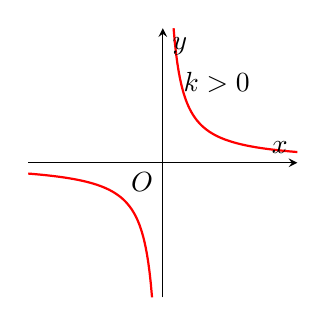
\begin{tikzpicture}
					\begin{axis}[
						axis lines=middle,
						xlabel={\(x\)}, ylabel={\(y\)},
						xmin=-5, xmax=5, ymin=-5, ymax=5,
						xtick=\empty, ytick=\empty,
						width=5cm, height=5cm,
						samples=100
						]
						\addplot[thick, red, domain=-5:-0.4] {2/x};
						\addplot[thick, red, domain=0.4:5] {2/x};
						\node at (axis cs:2,3) {\(k>0\)};
						\node at (axis cs:0,0) [below left] {\(O\)};
					\end{axis}
				\end{tikzpicture}
			\end{column}
			\begin{column}{0.6\textwidth}
				\textbf{解答：}\\
				（1）函数 \(y=\frac{k}{x}\) 的定义域为 \(D=\{x \mid x \neq 0\}\)，即 \((-\infty, 0) \cup (0, +\infty)\)。
				
				\vspace{0.2cm}
				（2）它的单调性如下（假设 \(k>0\) 为例）：\\
				\begin{itemize}
					\item 在 \((-\infty, 0)\) 上单调递减；
					\item 在 \((0, +\infty)\) 上单调递减。
				\end{itemize}
				\textbf{证明（以 \(k>0, x \in (0, +\infty)\) 为例）：}\\
				任取 \(x_1, x_2 \in (0, +\infty)\)，且 \(x_1 < x_2\)。
				\[ f(x_1) - f(x_2) = \frac{k}{x_1} - \frac{k}{x_2} = \frac{k(x_2 - x_1)}{x_1x_2} \]
				因为 \(0 < x_1 < x_2\)，所以 \(x_1x_2 > 0\)，\(x_2 - x_1 > 0\)。\\
				又因为 \(k>0\)，所以 \(f(x_1) - f(x_2) > 0\)，即 \(f(x_1) > f(x_2)\)。\\
				故在 \((0, +\infty)\) 上单调递减。同理可证 \(k<0\) 及其他区间的情况。
			\end{column}
		\end{columns}
	\end{frame}
	
\end{document}